\section{Fragen}
\subsection{Unterscheidung zwischen induzierter und spontaner  Photoemission}
Spontane und induzierte Emission unterscheiden sich sowohl in ihrer räumlichen als auch ihrer zeitlichen Abstrahlcharakteristik. \newline
So wird das Photon bei induzierter Emission in die gleiche Richtung emittiert wie das einfallende Photon. Bei der spontanen Emission jedoch werden durch Abregung ausgesendete Photonen isotrop in alle Raumrichtungen abgestrahlt. \newline
Die zeitliche Entwicklung der induzierten Emission ist abhängig von der Photonenzahl in dem Laserresonator, da mehr Photonen mehr Atome abregen können und es so zu einer höheren Emission kommt. Da die spontane Emission allerdings, wie der Name vermuten lässt, spontan verläuft und somit nur durch den Zufall bestimmt ist, bleibt die Emissionsrate hier im Großen zeitlich konstant und ist proportional zum Inversen der Lebensdauer des jeweiligen angeregten Zustandes.
\subsection{Beispiele für homogene und inhomogene Linienverbreiterung} 
Als Beispiel für eine homogene Linienverbreiterung kann die natürliche Linienbreite angeführt werden. Die Verbreiterung der Linie steht dabei in direktem Zusammenhang mit der Lebensdauer des angeregten Zustandes und beruht auf der Energie-Zeit-Unschärfe, die besagt, dass für einen Prozess, dessen zeitliche Dauer genau bestimmt werden kann, die Energie des Prozesses dementsprechend ungenau bestimmt werden kann. \newline
Eine inhomogene Linienverbreiterung stellt die Dopplerverbreiterung dar, der von der thermischen Bewegung der Atome innerhalb des Lasermediums und somit auf der Frequenzverschiebung durch den Dopplereffekt beruht. 
\subsection{Zwei - und Dreiniveausysteme}
Der Aufbau und die Funktionsweise eines Dreiniveau-Lasersystems wird im Folgenden dargestellt. \newline
Ein solches System hat ein Grundniveau mit der Energie E$_1$, das gleichzeitig das untere Laserniveau darstellt, ein oberes Laserniveau mit Energie E$_2$ und einem Pumpniveau mit der Energie E$_3$, wobei E$_3$>E$_2$ gilt. \newline
Um einen solchen Laser nun in Betrieb nehmen zu können, müssen die Elektronen aus dem Grundniveau in das Pumpsystem angeregt werden, indem dem System die Energie E$_3$-E$_1$ zugeführt wird. Von diesem Niveau gehen die Elektronen in einem schnellen, strahlungsfreien Übergang in das obere Laserniveau über und regen sich von diesem zunächst spontan, mit längerer Betriebszeit des Lasers induziert, in das untere Laserniveau, das in einem Dreiniveausystem dem Grundzustand entspricht, unter Emission des gewünschten Laserlichts ab. Damit es jedoch zu der benötigten Besetzungsinversion kommt und das obere Laserniveau ausreichend bevölkert ist, muss für die Lebensdauern der Niveaus E$_3$ E$_2$ und $\tau_{E_3} \ll\tau_{E_2}$ gelten, das Pumpniveau muss also schneller entvölkert werden als das obere Laserniveau bevölkert wird. \newline
Es ist zu bemerken, dass bei einem solchen System das Pumpniveau und das obere Laserniveau, anders als bei einem Zweiniveausystem, zwei unterschiedliche Niveaus sind. Genau aufgrund dieser Gleichheit der beiden Niveaus ist es, wie bereits in Abschnitt 2.1 angedeutet, nicht möglich einen Zweiniveau-Laser zu betreiben. Hier können durch pumpen problemlos bis zur Hälfte der Elektronenzahl Elektronen in das obere Laser - und gleichzeitig Pumpniveau angeregt werden. Da bei einem Zweiniveausystem jedoch die Energie zum Pumpen und für die induzierte Emission der gleichen Energie entspricht, ist sobald die Elektronen gleichmäßig auf beide Nivaus aufgeteilt sind, die Wahrscheinlichkeit ein Elektron aus dem unteren Niveau anzuregen genauso hoch wie eines aus dem oberen Niveau abzuregen. Durch Pumpen kann also höchstens die Hälfte der Elektronen angeregt werden, was für eine Besetzunginversion, die für einen Laser benögtigt wird jedoch nicht ausreicht. Bezieht man nun noch spontane Emission mit ein, die trotz allem auch stattfindet, so kommt es in realen Zweiniveausystemen nicht einmal zur Anregung der Hälfte der Elektronen, die Besetzungsinversion kann also nie erreicht werden, womit der Betrieb eines Lasers mit einem solchen System nicht möglich ist.
\subsection{Beschränkung der Pumpleistung}
Die maximale Pumpleistung ist durch die stimulierte Emission aus dem Pumpniveau direkt in zurück in das Grundniveau beschränkt. Das Grund - und Pumpniveau lassen sich nämlich, wenn alle Niveaus dazwischen vernachlässigt werden, als Zweiniveausystem interpretieren. Wie in 5.3. beschrieben, kann bei einem solchen System höchstens die Hälfte der Elektronen in das obere Niveau angeregt werden, da ab diesem Punkt die Wahrscheinlichkeit ein Elektron anzuregen genau der Wahrscheinlichkeit entspricht eines abzuregen. \newline
Um zu verhindern, dass es so weit kommt, müssen also die strahlungsfreien Prozesse schnell genug stattfinden, um das Pumpniveau in das obere Laserniveau zu entvölkern, bevor das nächste Pumpphoton auf das Atom trifft, so dass es gar nicht erst zu einer Sättigung des Pumpniveaus kommt. 
\subsection{Modenabstand für L=1}
Aus Gleichung (\ref{equ:resonance}) erhält man wie bereits genannt
\begin{equation*}
	\triangle\omega=\frac{c\pi}{L}=2\pi\triangle f
\end{equation*}
Setzt man nun ein, erhält man $\triangle\omega$=942.48 MHz. Vergleicht man dies mit der Frequenz eines 1047nm-Lasers, wie er in dem Versuch verwendet wurde, so erhält man
\begin{equation*}
\frac{\omega}{\triangle\omega}=\frac{1.8\cdot10^{15}\text{Hz}}{942.48\cdot10^6 \text{Hz}}\approx2\cdot10^6
\end{equation*}
Die Frequenz des Lasers ist also sechs Größenordnungen größer als der Frequenzabstand zweier benachbarter Moden, das heißt die Moden liegen eng beieinander. Dies lässt sich auch am Wellenlängenabstand zweier Moden sehen, für den sich nach Gleichung (\ref{umrechnung}) und mit $\lambda_1\approx\lambda2$=1047nm
\begin{equation*}
\triangle\lambda=5.48\cdot10^{-13}\text{m}=0.548 \text{pm}
\end{equation*}
\subsection{Auswirkung der spektralen Halbwertsbreite auf die Impulsdauer}
Nach Gleichung (\ref{impulsbandbreite}) muss im Bereich des Idealwertes von 0.441 bei einer kleinen Bandbreite des Lasers die Dauer dementsprechend länger werden. Andersrum kann für ein umso breiteres Laserspektrum ein umso kürzerer Puls erzeugt werden. Hierfür spielt die Anzahl der gekoppelten Moden eine wichtige Rolle, da sich mit steigender Anzahl der gekoppelten Moden die Impulsdauer verringert.
\subsection{Nichtlineare Polarisation auf atomarer Ebene}
Elektronen in einem Atom spüren ein Potential, dessen Verlauf in Abhängigkeit des Abstandes vom Kern schematisch in Abbildung \ref{Potential} abgebildet ist. 
\begin{figure}[H]
	\begin{center}
		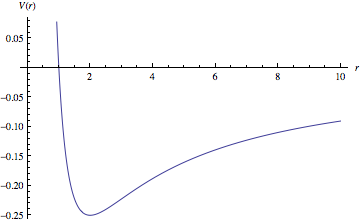
\includegraphics[scale=.75]{Bilder/Potential.png}
		\caption{Potential eines Elektrons im Atom}
		\label{Potential}
	\end{center}
\end{figure}
Legt man nun ein elektrisches Feld an das Atom an, so werden die Elektronen um ihre Gleichgewichtslage im Mininum des Potentials ausgelenkt. Ist das elektrische Feld dabei klein genug, so kann dass Potential in Umgebung des Minimums quadratisch annähern. Man erhält also eine Rückstellkraft proportional zur Auslenkung x, die wiederrum proportional zu dem angelegten elektrischen Feld sind. Nutzt man nun die Definiiton des Dipolmoments p
\begin{equation}
	p=xq
\end{equation}
mit q der Ladung, so erhält man ein Dipolmoment proportional zu E. Da die Polarisation eines Körpers lediglich dessen Dipolmomentdichte beschreibt ist sie somit linear für kleine Felder. \newline
Ist das angelegt Feld nun immer größer, so werden die Elektronen immer stärker aus ihrer Gleichgewichtslage ausgelenkt und aus Abbildung (\ref{Potential}) ist leicht ersichtlich, dass eine quadratische Näherung des Potentials nicht mehr ausreicht. Dadurch erhält man in der Rückstellkraft Beiträge höherer Ordnungen der Auslenkungen, wodurch auch das Dipolmoment nicht mehr linear wird, sondern mit höherer Feldstärke höhere und höhere Ordnungen berücksichtigt werden müssen. Aus dieser Nichtlinearität des Dipolmoments für hohe Felder folgt dann auch direkt eine Nichtlinearität der Polarisation. 
\subsection{Gleichheit der Brechungsindizes von Grund - und Oberwelle}
Da die Lichtgeschwindigkeit in einem Medium nur von dessen Brechungsindex bestimmt wird, müssen die Brechungsindices der Grund - und der Oberwelle indentisch sein, um eine effektive Erzeugung letzterer zu garantieren. \newline
Sind die Brechungsindizes für beide gleich, so bewegen sich beide Wellen gleich schnell durch den Kristall, für die Wellenvektoren beider Wellen gilt $\triangle$k=2k$_\omega$-k$_{2\omega}$=0. Die Fundamentale k$_\omega$ erzeugt nun am Ort x im Kristall eine Oberwelle k$_{2\omega}$. Wird nun eine weiter Oberwelle am Ort x-$\triangle$x erzeugt, so ist diese mit der am Ort x erzeugten Oberwelle in Phase und beide können konstruktiv interferieren
Wären die Brechungsindices nicht identisch, so bewegt sich eine der Wellen schneller durch den Kristall als die andere und eilt dieser damit voraus. Somit ist eine später erzeugte Oberwelle im Allgemeinen nicht in Phase mit einer früheren, es kommt nicht zu konstruktiver Interferenz. 
\begin{figure}
	\centering
	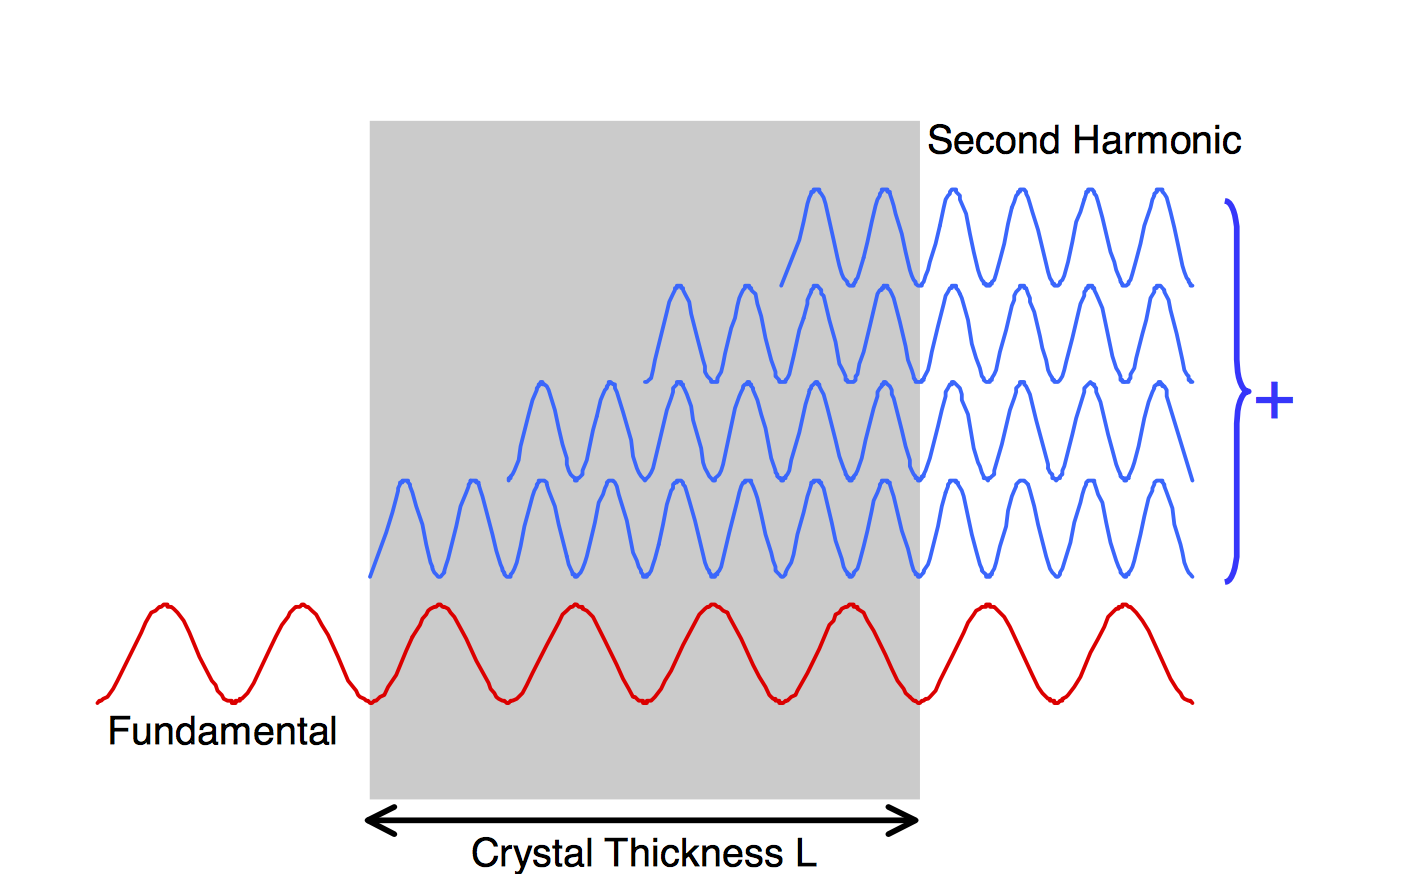
\includegraphics[width=0.7\linewidth]{Bilder/Oberwelle}
	\caption{Schematische Darstellung der Oberwellenerzeugung}
	\label{fig:oberwelle}
\end{figure}
Die ist in Abbildung \ref{fig:oberwelle}\footnote{de Dood, M.J.A. (2006), S. 5}schematisch dargestellt. Hier sind die Brechungsindizes für Fundamentale (in rot) und Oberwellen (in blau) gleich und jede erzeugte Oberwelle ist mit der vorigen in Phase. Wäre nun beispielsweise die Fundamentale schneller, so wären die oberen Oberwellen in der Abbildung, also die später erzeugten relativ zu den vorderen verschoben. Es kommt somit zu einer Phasenverschiebung und damit zu keiner konstruktiven Interferenz
\subsection{Bestimmung der Impulsform aus Autokorrelationsmessung}
Wie Gleichung (\ref{eq:Autokorr}) leicht anzusehen ist, ist die Autokorrelationsfunktion symmetrisch bezüglich der y-Achse. Das heißt man kann die genaue Form des Laserpulses nicht aus der Autokorrelationsmessung bestimmen, da nicht eindeutig bestimmt werden kann, ob der ursprüngliche Puls nur zum dem Ursprung linksseitigen oder nur dem rechtsseitigen Teil des Graphen beigetragen hat und der jeweils andere lediglich durch Spiegelung aufgrund der Symmetrie entstanden ist oder gar der gesamte Graph den Puls darstellt.
%%% mode: latex
%%% TeX-master: "../Laser"
%%% End:
